\documentclass{article}

\usepackage[preprint]{nips_2018}
% to avoid loading the natbib package, add option nonatbib:
% \usepackage[nonatbib]{nips_2018}

\usepackage[utf8]{inputenc} % allow utf-8 input
% \usepackage[T1]{fontenc}    % use 8-bit T1 fonts
\usepackage{hyperref}       % hyperlinks
\usepackage{url}            % simple URL typesetting
\usepackage{booktabs}       % professional-quality tables
\usepackage{amsfonts}       % blackboard math symbols
\usepackage{nicefrac}       % compact symbols for 1/2, etc.
\usepackage{microtype}      % microtypography
\usepackage{amsmath}
\usepackage{float}
\usepackage{graphicx}
\usepackage{algorithm}
\usepackage{algpseudocode}
\usepackage{cleveref}       % this package must be loaded at the last
\usepackage{subcaption}


\title{Lab1 Report}

\author{
  Chun Hung Lin \\
  \texttt{chlin3@kth.se}
  \And
  Yini Yang \\
  \texttt{yiniy@kth.se}
}

\begin{document}
\maketitle

% Quesiton 1
\section{Problem 1: The Maze and the Random Minotaur}
\subsection{Formulate the problem as an MDP}
This problem can be formulated as an MDP with finite horizon.
\newline

\textbf{State space:} \\
Here we use a pair of positions in the maze as a state. The state space $S$ can be described as follows:
$$S=\{S_i=(x_p,y_p,x_m,y_m)|i=0,\cdots,3136\}, \quad x_p,x_m\in [0,6],\  y_p,y_m\in [0,7]$$
where $(x_p,y_p)$ refers to the position of the person, while $(x_m,y_m)$ is the position of the Minotaur.
Here we can divide this state space into four part:
$$S=S_{unavailable}\cup S_{available}\cup S_{dead}\cup S_{escape}$$
where $S_{unavailable}=\{(x_p,y_p)\in wall\}$ refers to the states where the person is in the wall. 
$S_{dead}=\{S_i|x_p=x_m,y_p=y_m\}$ corresponds to the states where the person and minotaur are in the same position. 
$S_{escape}=\{S_i|(x_p,y_p)=exit,(y_p,y_m)\neq exit\}$ includes the states at which the person succeeds escaping.
And both $S_{dead}, S_{escape}$ are absorbing states.
\newline

\textbf{Action space:} \\
In this problem, the minotaur follows a random walk. The action space for the person is as below:
$$A=\{\textup{Up},\textup{Down},\textup{Left},\textup{Right},\textup{StandStill}\}$$
\newline

\textbf{Reward:} \\
The reward can be formulated as a function of $r: S\times A\rightarrow \mathbb{R}$.
$$r(s,:)=\left\{\begin{aligned}
 10 \quad &s\in S_{escape} \\
 -1 \quad &s\in S_{dead} \\
 0 \quad &\textup{otherwise}
\end{aligned}\right.$$
When the state is in $S_{escape}$, no matter what actions the person take, the reward will always be 10. 
While the state is in $S_{dead}$, the punishment will be $-1$ for whatever actions. 
For other available movement, there will be no reward or punishment.
\newline

\textbf{Transition probability:} \\
For the person, the policy is deterministic. In other words, given the current position and the action, the next position of the person is deterministic.
So for the state transition, the uncertainty comes from the minotaur. Thus the transition probability can be formulated as follows:
$$P_t(S_j|S_i,a)=\left\{\begin{aligned}
  &\frac{1}{|\textup{Aja}(S_{i_M})|} \quad &S_{j_M}\in \textup{Aja}(S_{i_M}) \\
  &1 \quad &S_i\in S_{dead}\cup S_{escape} \\
  &0 \quad &\textup{otherwise}
\end{aligned}\right.$$
where $S_{i_M}=(x_{i_m},y_{i_m})$ means the minotaur's position at state $i$, and $\textup{Aja}(S_{i_M})$ is the set of adjacent positions to $S_{i_M}$.
And when the environment has reached the absorbing state, it will always stay in this state.
\newline

\textbf{Objective funcion:} \\
This MDP is under a finite time horizon $T$. Thus the objective function can be formulated as the total rewards obtained in $T$ steps:
$$G_T=\mathbb{E}\left\{\sum_{t=0}^T r_t(S_t,a_t)\right\}$$

\subsection{Solve the problem for T=20}
One generated solution has been shown in Figure \ref{solution}.
The red arrows correspond to the person's route, while the blue ones refer to the minotaur's route.
In this solution, the person succeeds escaping when $t=17$.
\begin{figure}[h]
  \centering
  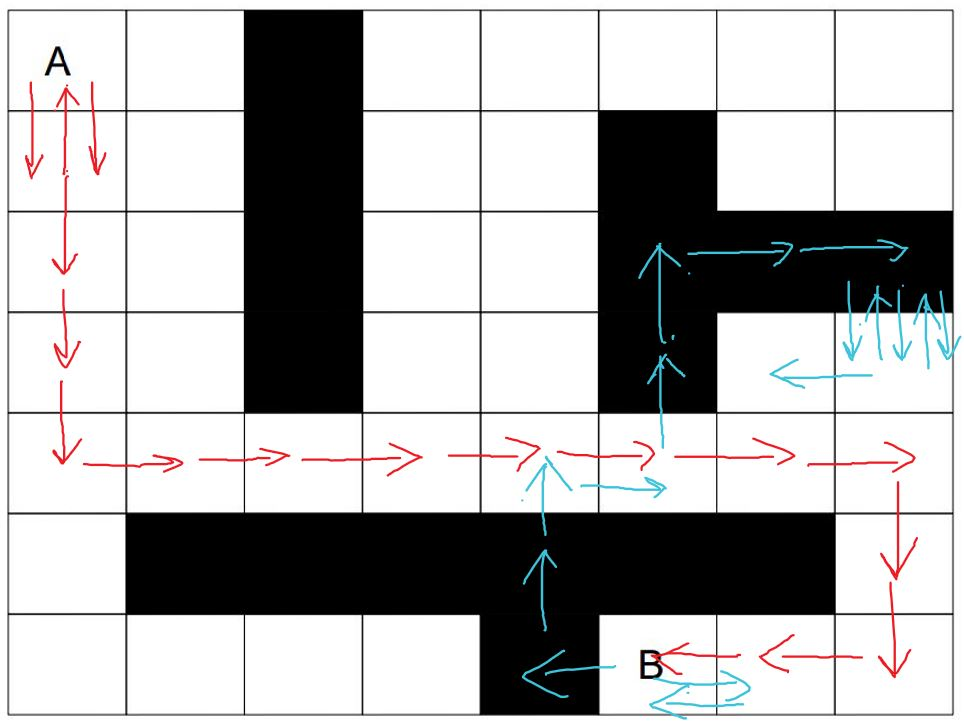
\includegraphics[scale=0.5]{solution.jpg}
  \caption{A generated solution for T=20}
  \label{solution}
\end{figure}


\subsection{Modify MDP with infinite time horizon}
Under this condition, the time horizon is no longer finite. Instead, $T$ is infinite and follows the following geometric distribution:
$$P(T=t)=(1-p)^tp, \quad t=0,1,\cdots$$ 
where $p=\frac{1}{30}$. Therefore, when $t$ is increasing, the probability is decreasing. 
Thus, we can re-formulate this problem as a MDP with infinite time horizon and discounted rewards. The objective function is changed into:
$$G_{\gamma}=\mathbb{E}\left\{\sum_{t=0}^{\infty}\gamma^t r_t(S_t,a_t)\right\}$$
where $\gamma=1-p=0.97$.
Other settings for this MDP are the same as before. And now we need to use the value iteration algorithm to obtain the optimal policy.

% Quesiton 2

% Quesiton 3
\section{Quesiton 3}

% Quesiton 4
\section{Quesiton 4}
\end{document}
